
% ------------------------ Prototype ------------------------

\section*{APPENDIX A - Prototype \label{sec:proto}}
\addcontentsline{toc}{section}{APPENDIX A - Prototype}


\begin{comment}

    Provide the filtered part of RM showing selected features for prototype building. State the detailed steps of compilation, execution and setups. Specify prototype details showing codes, screens, test data, sample output and detailed steps of compilation, execution and setups (if any).

\end{comment}

% ---------- Start the prototype appendix
    
\begin{figure}[h!]  
    \centering
    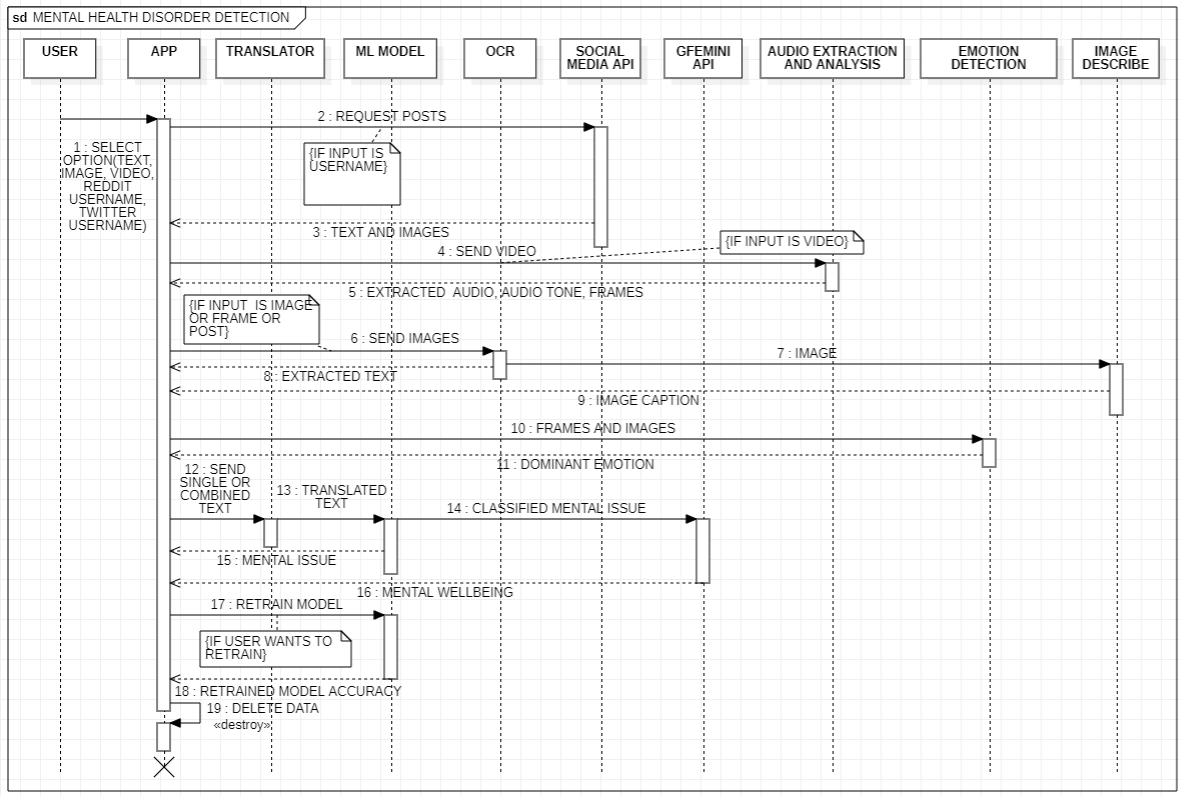
\includegraphics[width=1.0\textwidth]{Images/Sequence Diagram.png}  
    \caption{Sequence Diagram of the Application}
    \label{012i}  % Label for referencing the figure
\end{figure}

\noindent
Below are some screenshots from the web application.

\begin{figure}[h!]  
    \centering
    
\includegraphics[width=1.0\textwidth]{App Images/01 Interface.png}  
    \caption{Website with all options}
    \label{01i}  % Label for referencing the figure
\end{figure}

\begin{figure}[h!]  
    \centering
    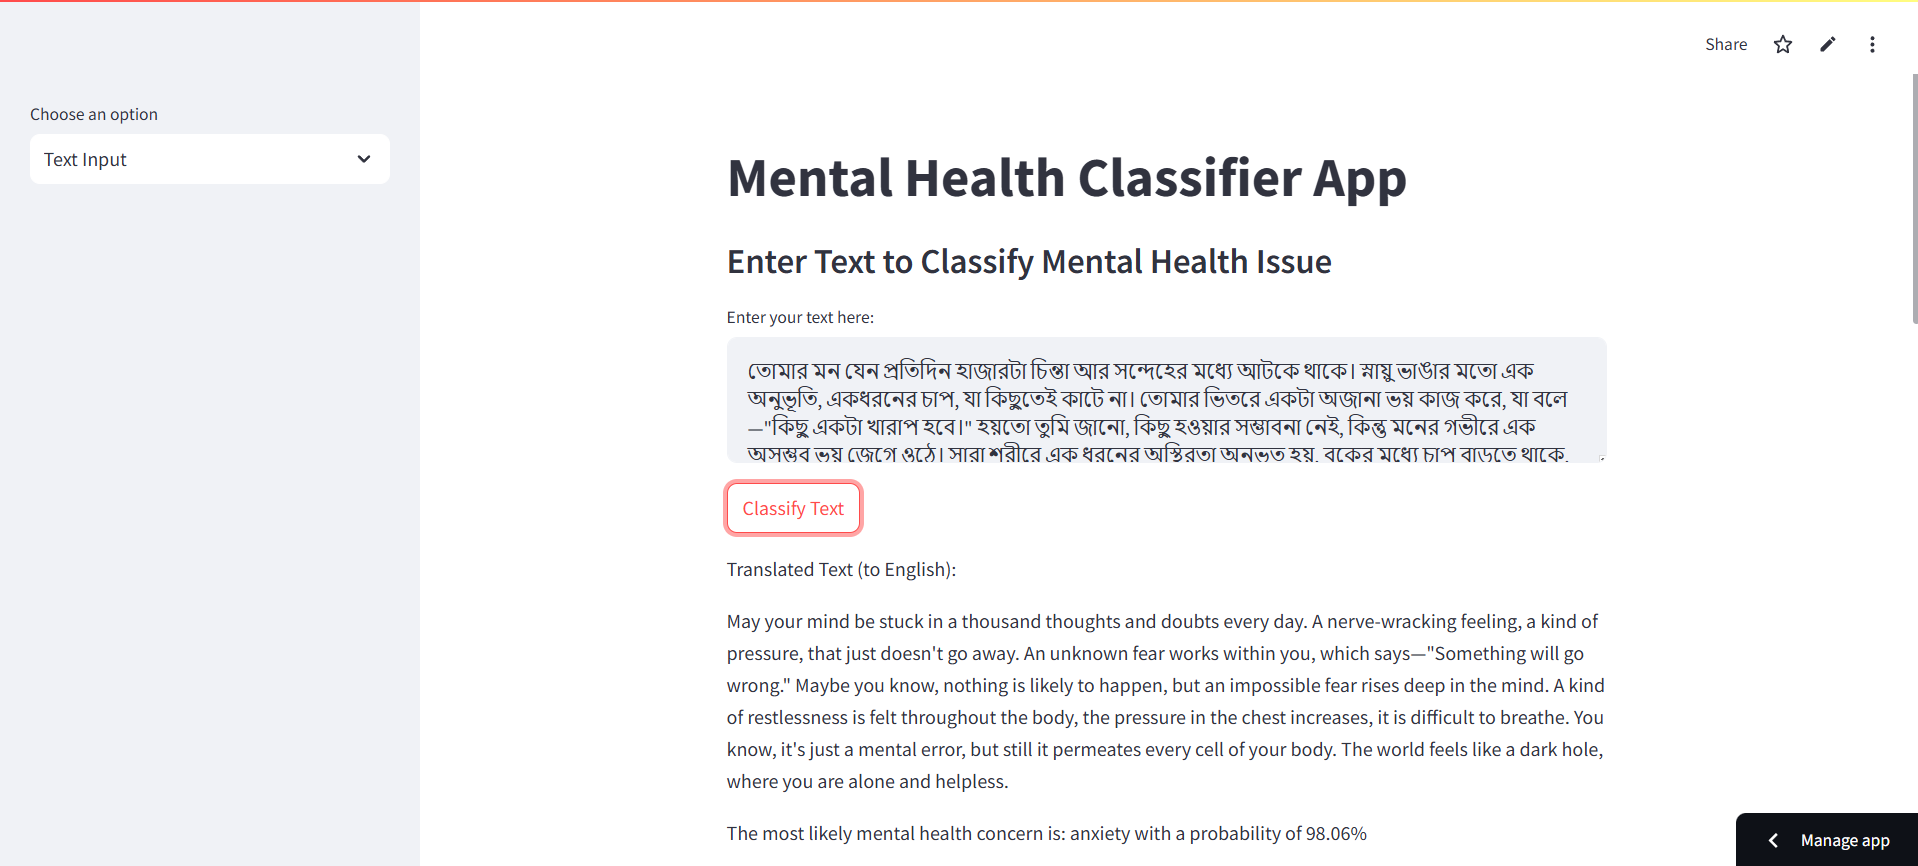
\includegraphics[width=0.8\textwidth]{App Images/02 Interface.png}  
    \caption{Entering Text for classification}
    \label{02i}  % Label for referencing the figure
\end{figure}

\begin{figure}[h!]  
    \centering
    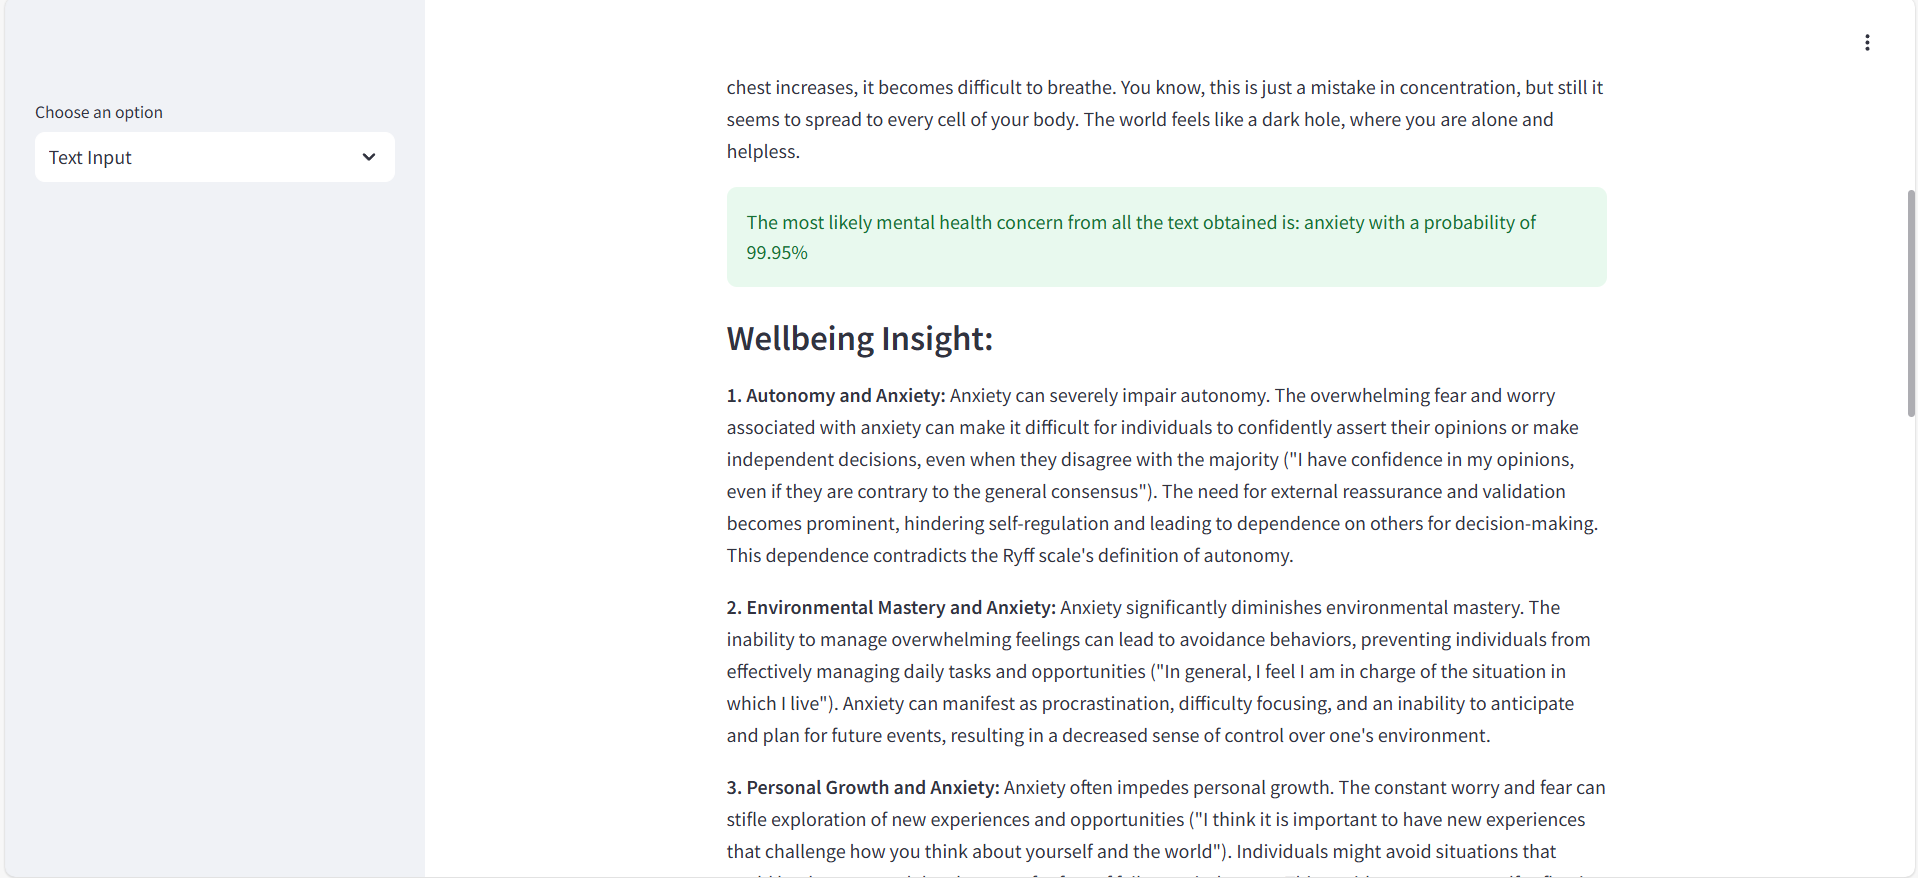
\includegraphics[width=0.8\textwidth]{App Images/03 Interface.png}  
    \caption{Text Classification Result}
    \label{03i}  % Label for referencing the figure
\end{figure}



\begin{figure}[h!]  
    \centering
    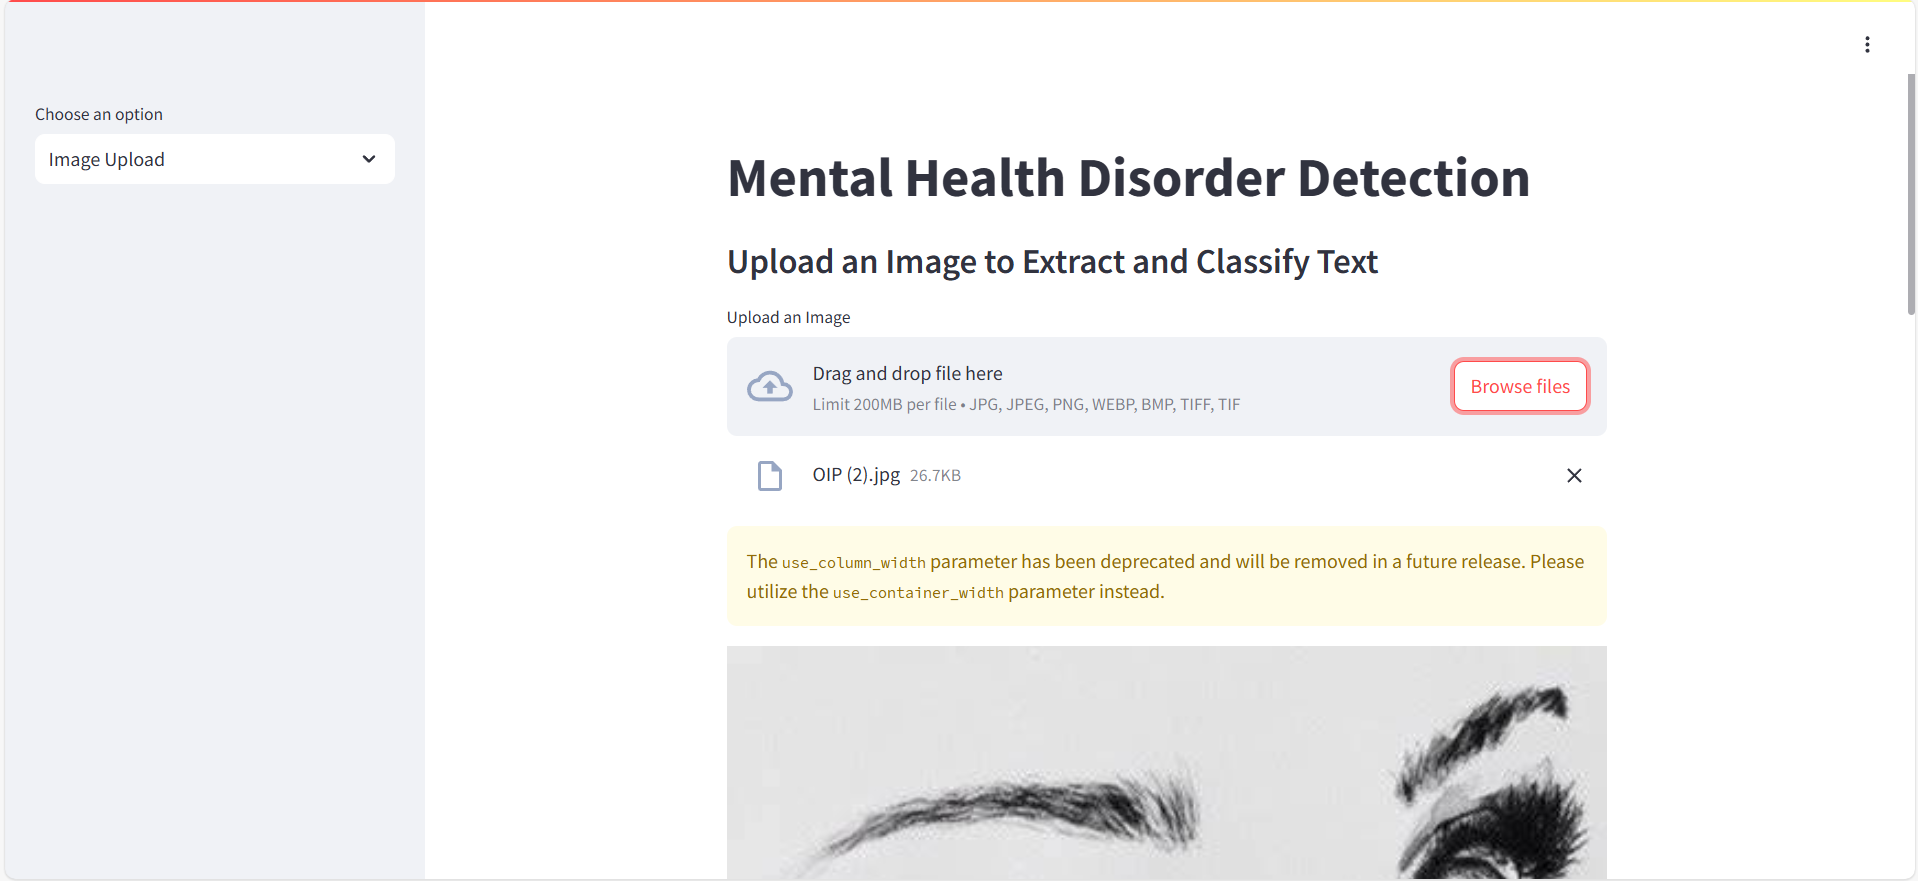
\includegraphics[width=0.8\textwidth]{App Images/04 Interface.png}  
    \caption{Upload Image}
    \label{04i}  % Label for referencing the figure
\end{figure}

\begin{figure}[h!]  
    \centering
    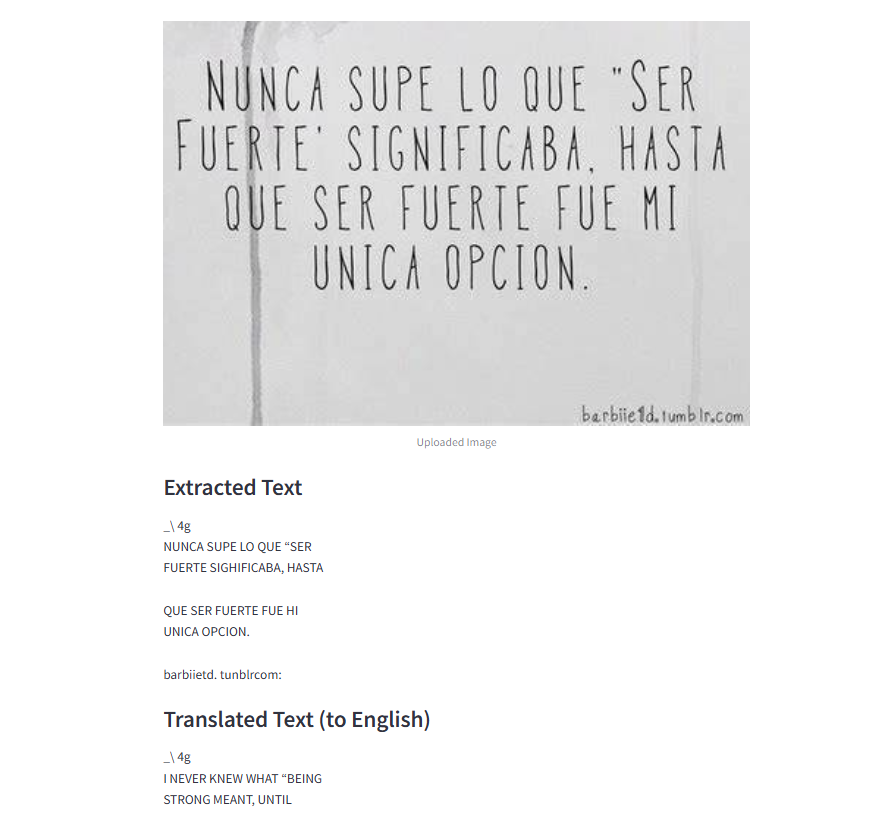
\includegraphics[width=0.8\textwidth]{App Images/05 Interface.png}  
    \caption{Image Classification Result}
    \label{05i}  % Label for referencing the figure
\end{figure}


\begin{figure}[h!]  
    \centering
    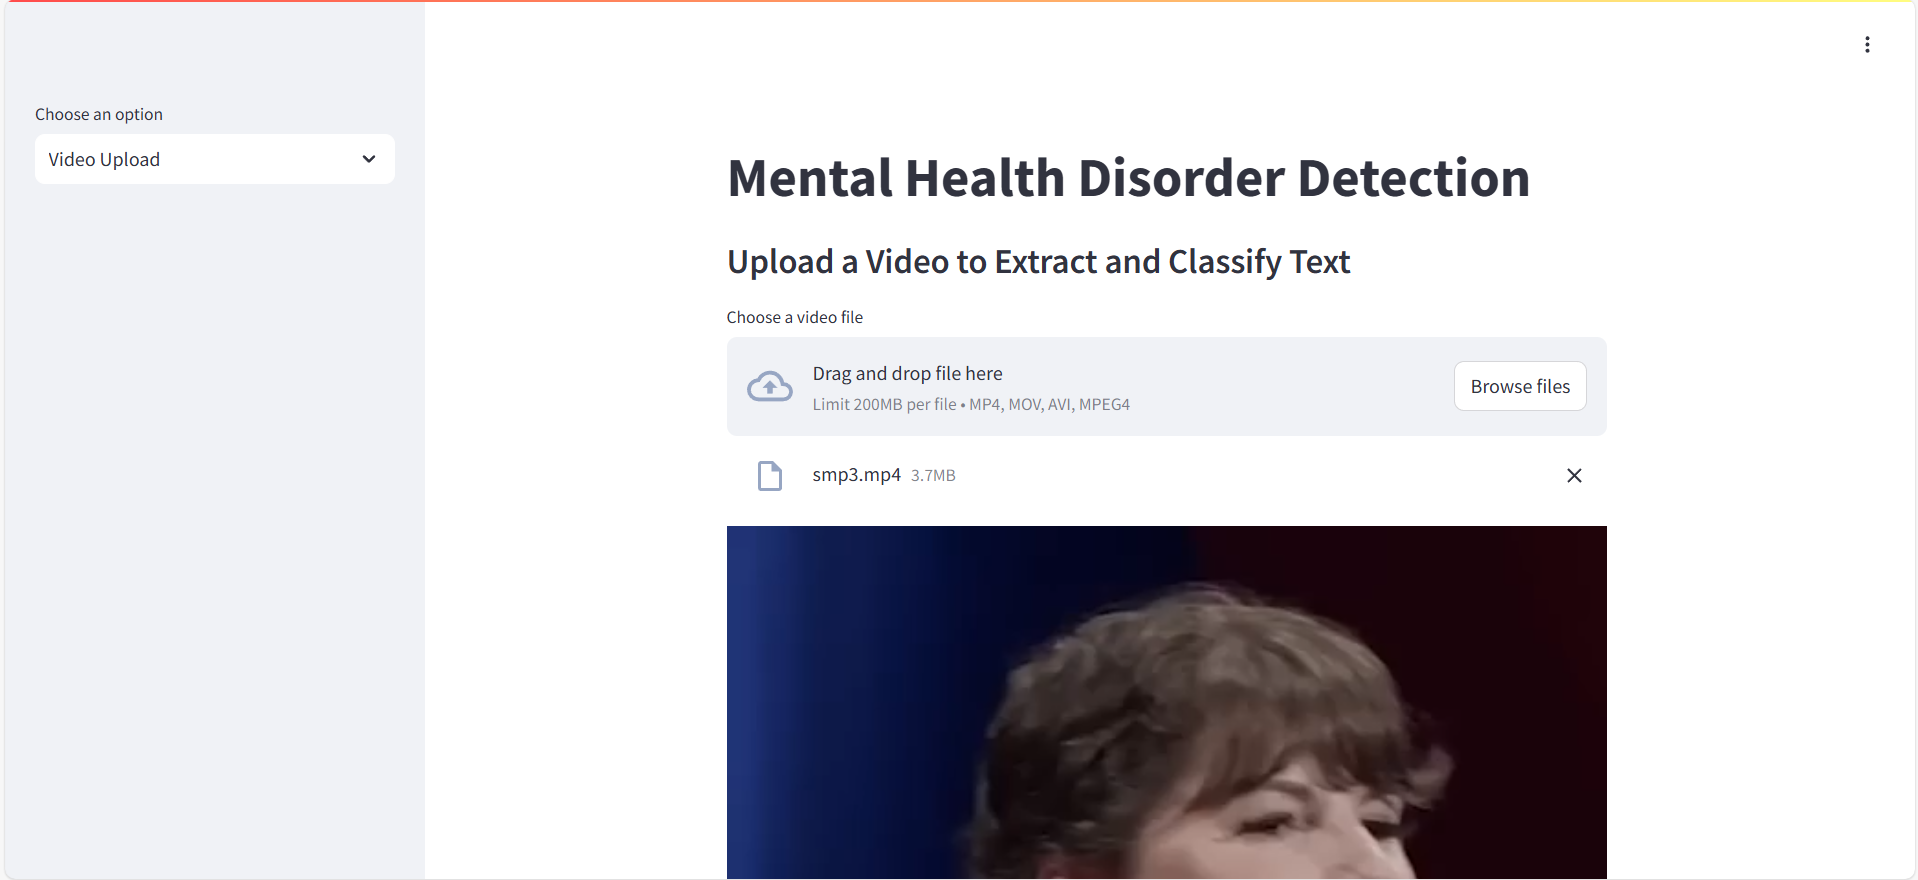
\includegraphics[width=0.8\textwidth]{App Images/12 Interface.png}  
    \caption{Upload Video}
    \label{06i4}  % Label for referencing the figure
\end{figure}

\begin{figure}[h!]  
    \centering
    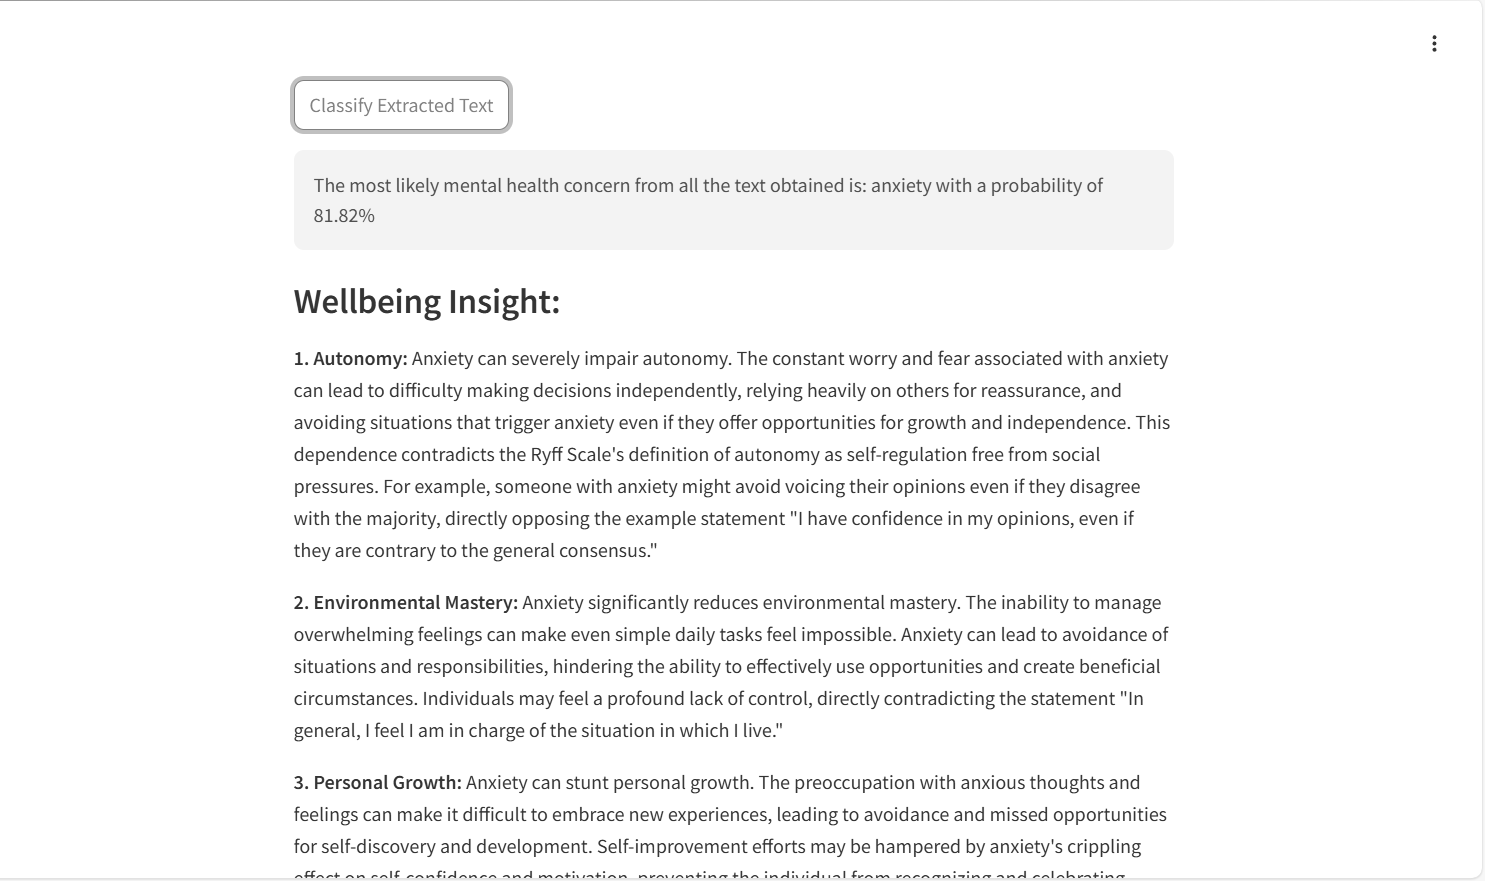
\includegraphics[width=0.8\textwidth]{App Images/13 Interface.png}  
    \caption{Video Classification Result}
    \label{06i}  % Label for referencing the figure
\end{figure}

\begin{figure}[h!]  
    \centering
    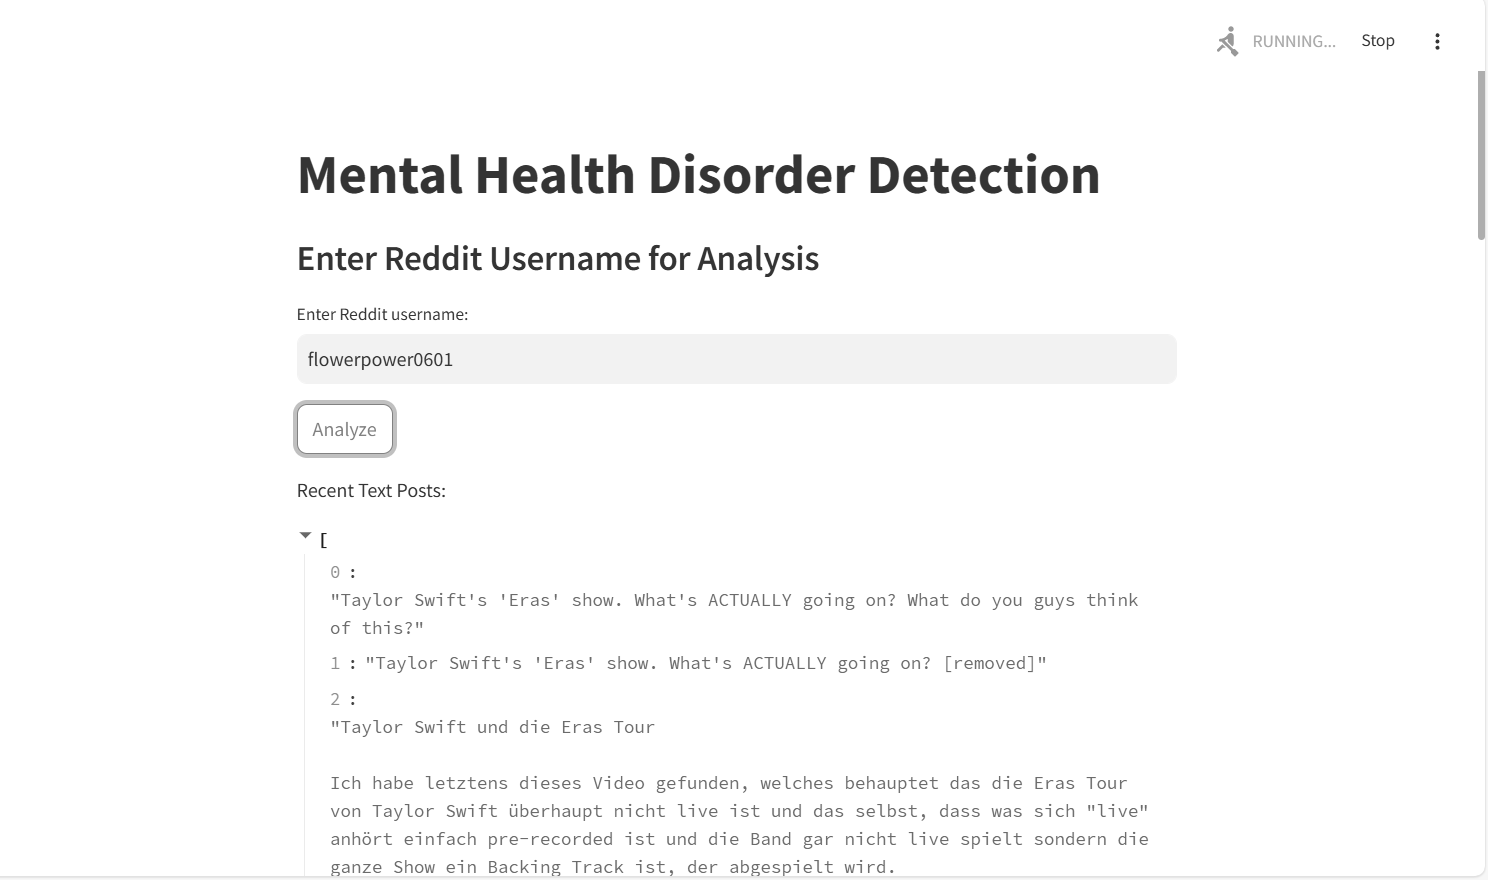
\includegraphics[width=0.8\textwidth]{App Images/06 Interface.png}  
    \caption{Reddit User Analysis}
    \label{07i}  % Label for referencing the figure
\end{figure}

\begin{figure}[h!]  
    \centering
    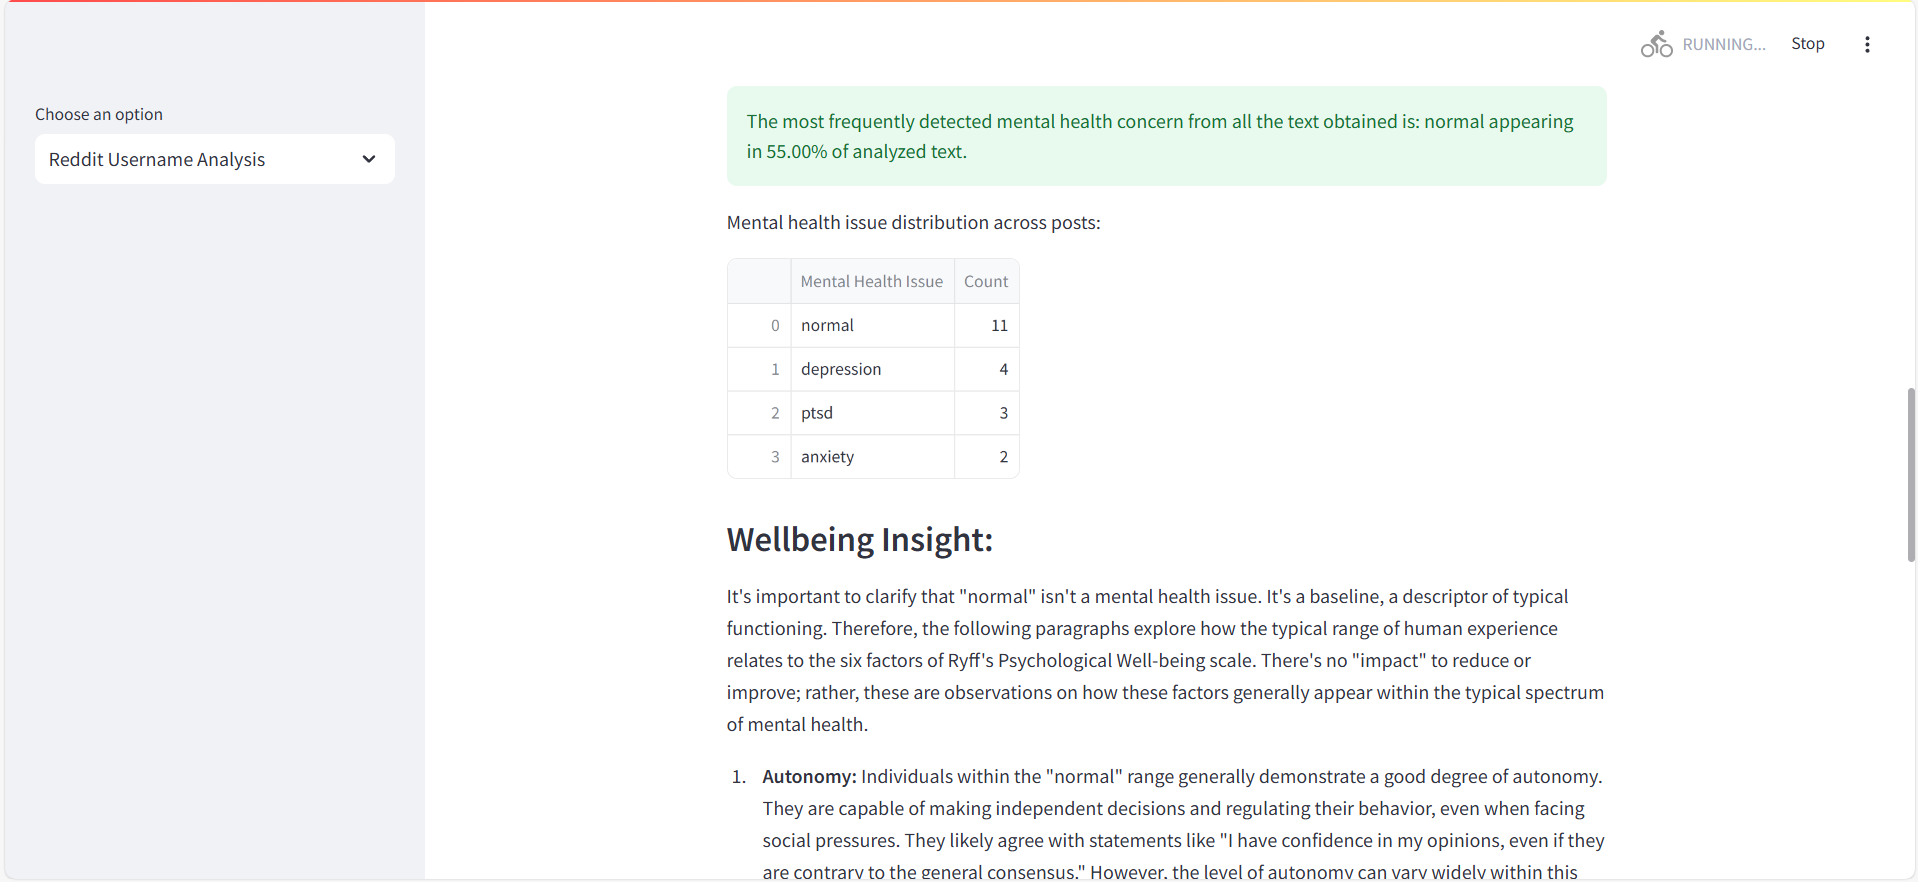
\includegraphics[width=0.8\textwidth]{App Images/07 Interface.png}  
    \caption{Result from Reddit Posts Analysis}
    \label{08i}  % Label for referencing the figure
\end{figure}


\begin{figure}[h!]  
    \centering
    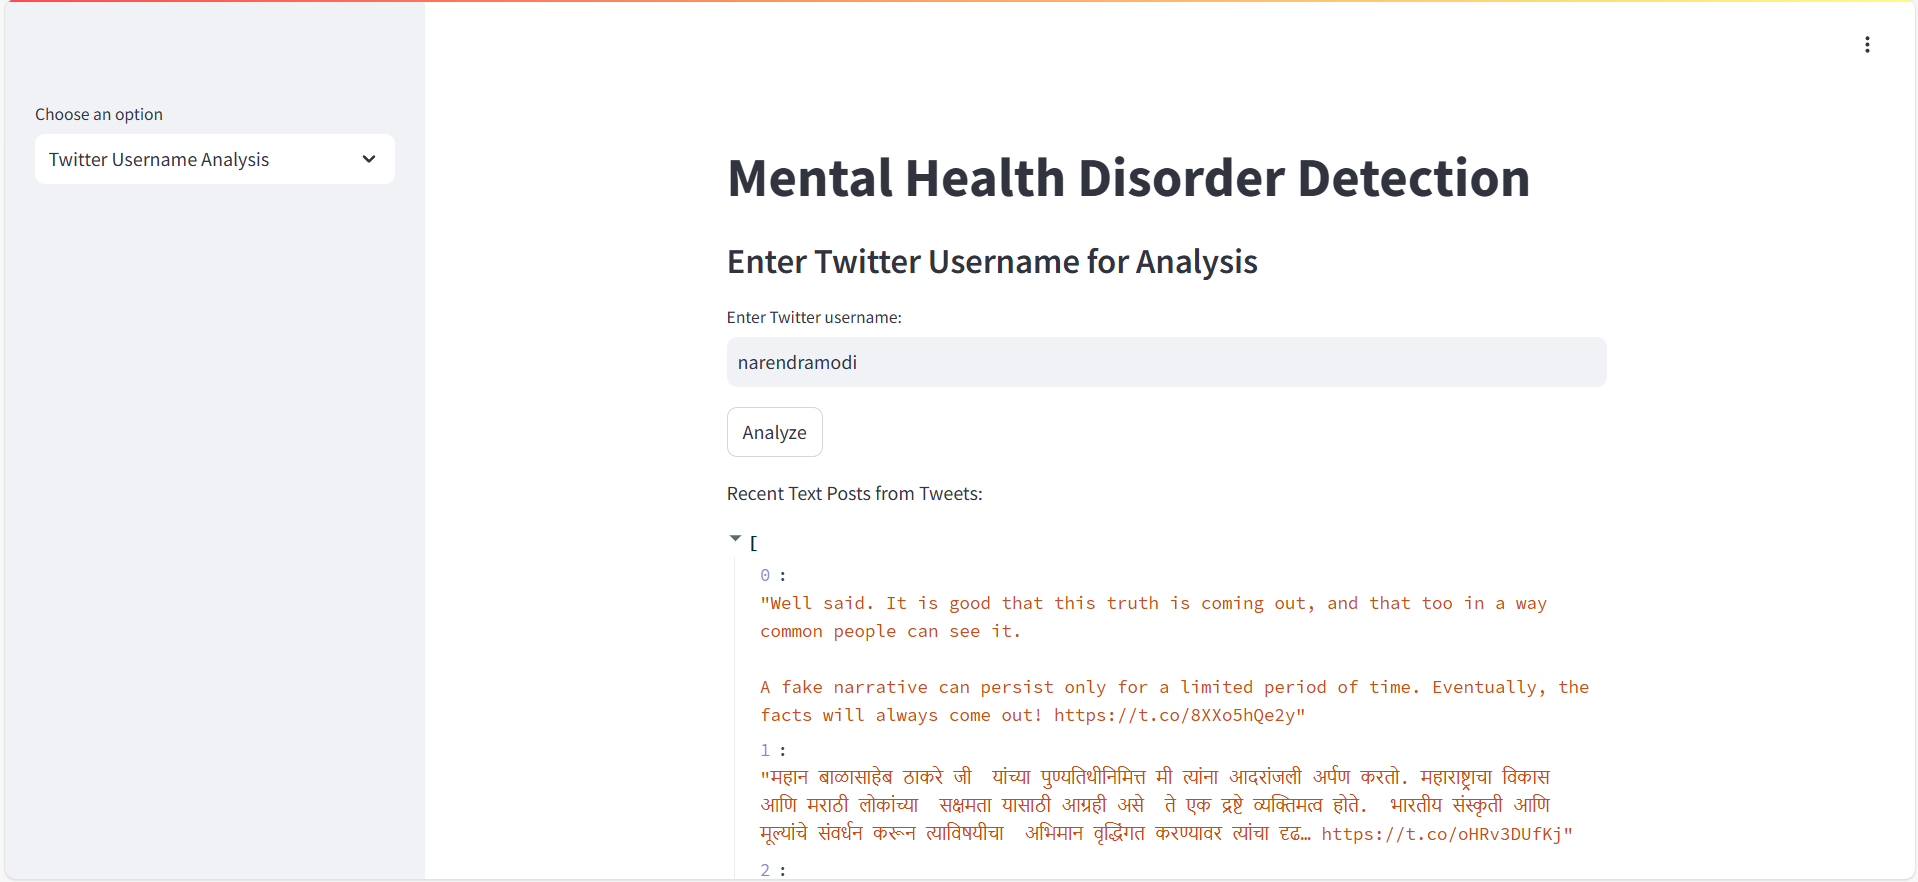
\includegraphics[width=0.8\textwidth]{App Images/08 Interface.png}  
    \caption{Twitter User Analysis}
    \label{09i}  % Label for referencing the figure
\end{figure}

\begin{figure}[h!]  
    \centering
    
\includegraphics[width=0.8\textwidth]{App Images/10 Interface.png}  
    \caption{Result from Twitter Posts Analysis}
    \label{10i}  % Label for referencing the figure
\end{figure}

\begin{figure}[h!]  
    \centering
    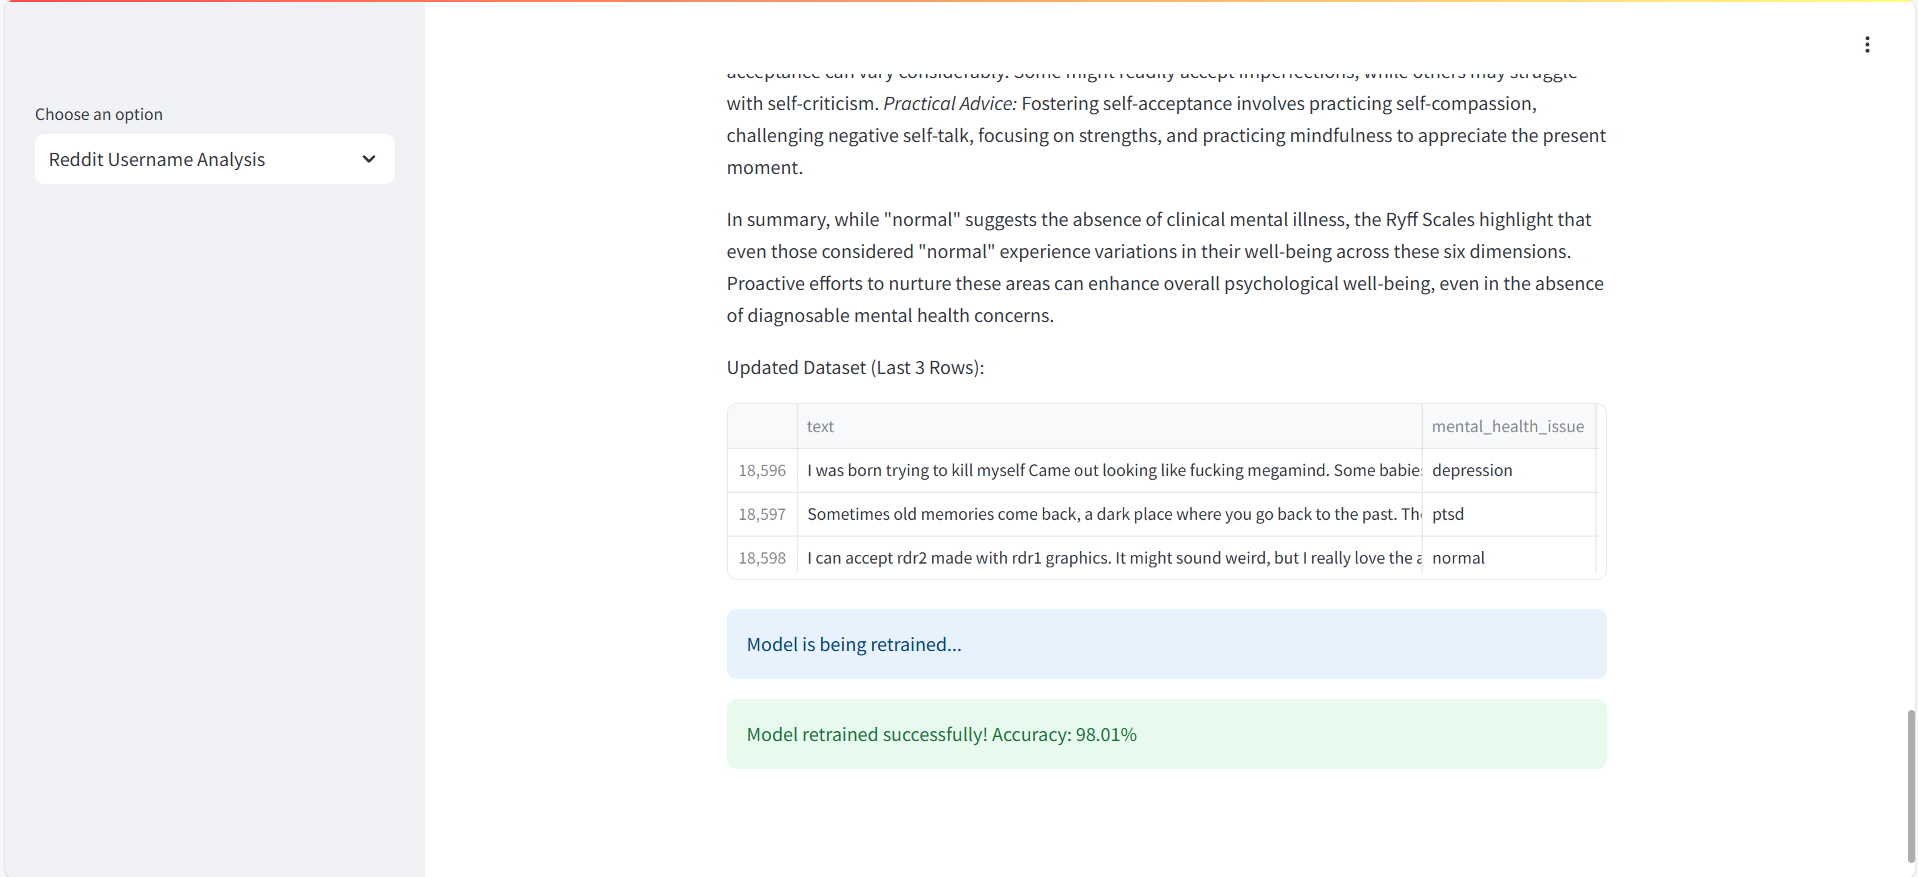
\includegraphics[width=0.8\textwidth]{App Images/17 Interface.png}  
    \caption{Result from Reddit Analysis and Model Retraining}
    \label{10i}  % Label for referencing the figure
\end{figure}

\begin{figure}[h!]  
    \centering
    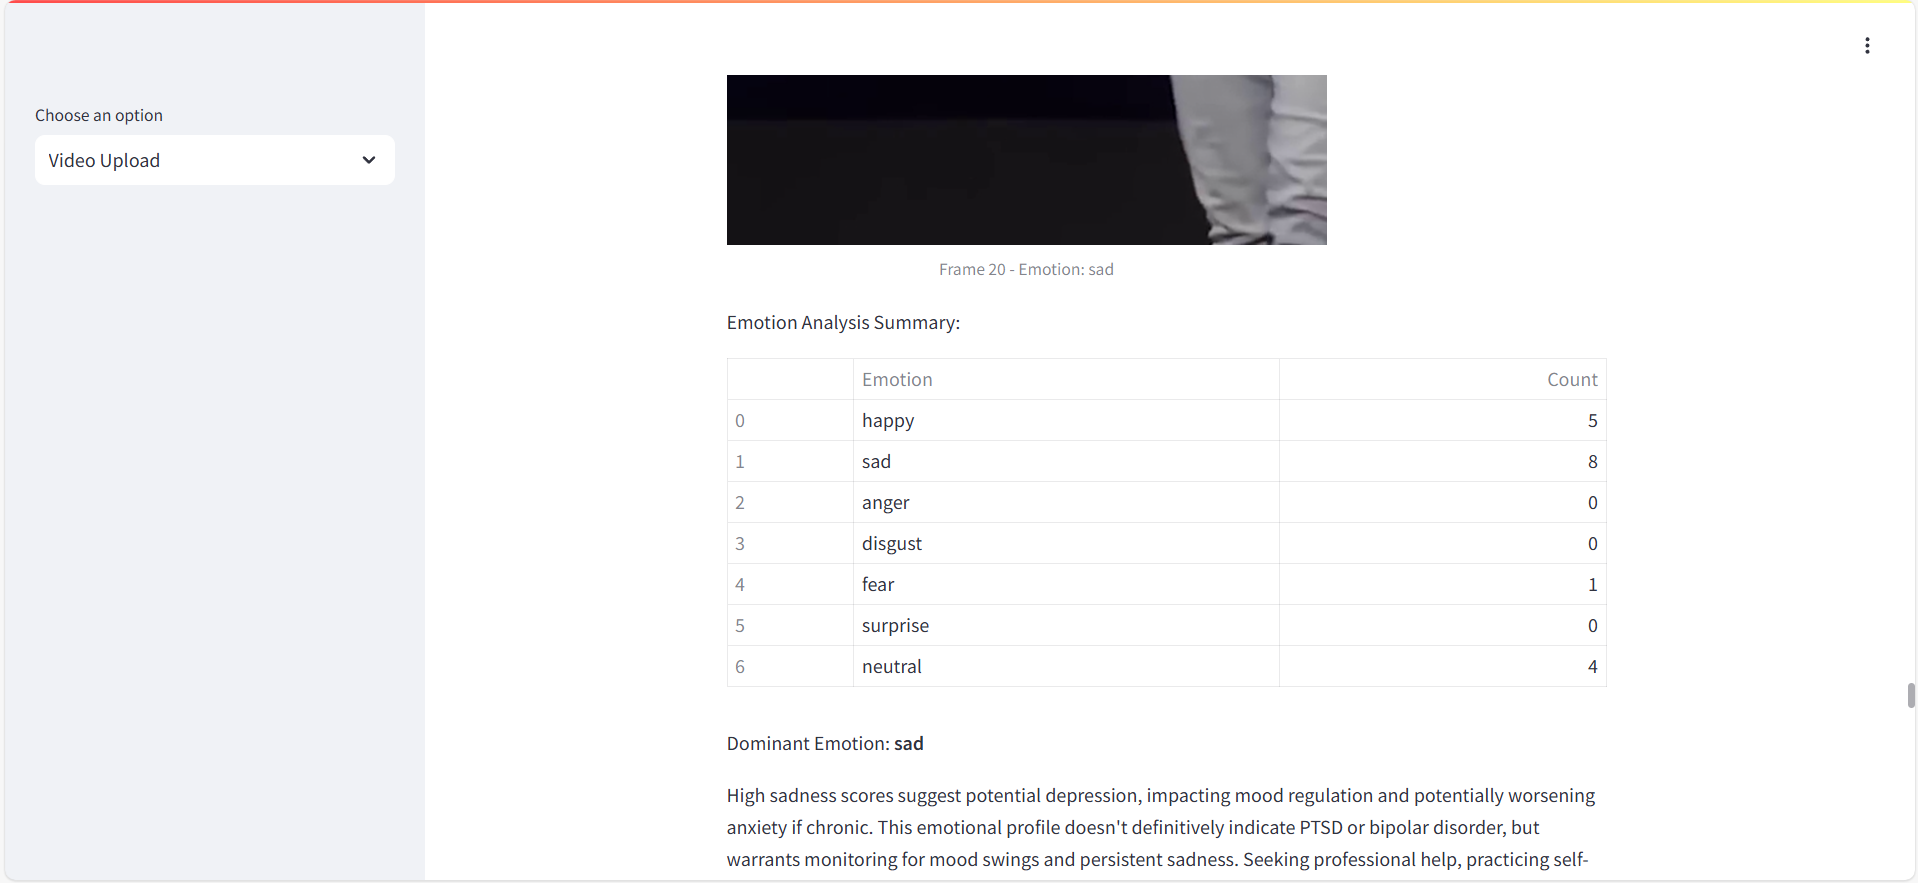
\includegraphics[width=0.8\textwidth]{App Images/12-1 Interface.png}  
    \caption{Result from the emotion analysis of facial expression}
    \label{10i23}  % Label for referencing the figure
\end{figure}

\begin{figure}[h!]  
    \centering
    
\includegraphics[width=0.8\textwidth]{App Images/18 Interface.png}  
    \caption{Generate Image Caption}
    \label{10i234}  % Label for referencing the figure
\end{figure}   

\begin{figure}[h!]  
    \centering
    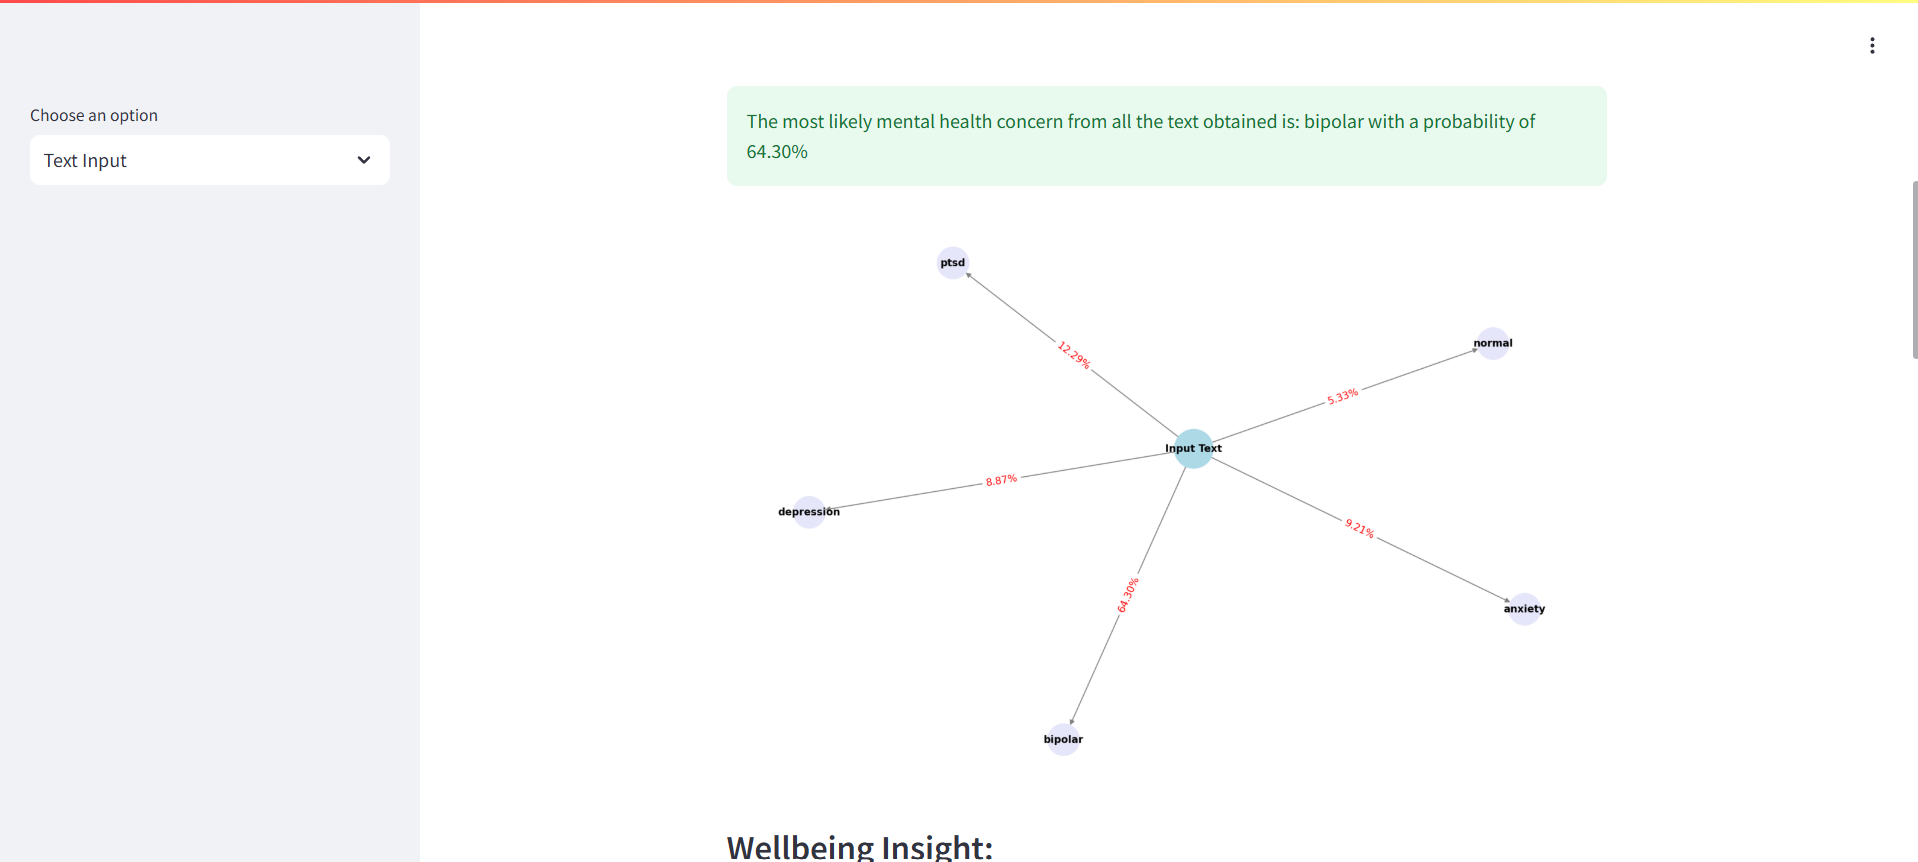
\includegraphics[width=0.8\textwidth]{App Images/19 Interface.png}  
    \caption{Knowledge Graph from classification}
    \label{10i23445}  % Label for referencing the figure
\end{figure}  







% ----------------------- Prototype ends -------------------


\begin{comment}

    \section*{APPENDIX B - Paper publications (optional) \label{sec:pubs}}
\addcontentsline{toc}{section}{APPENDIX B - Paper publications (optional)}
If any of your related paper(s) were published in a standard journal / presented in a recognized conference, mention the same including communication on your paper(s) acceptance / publishing note. You should also show appropriate documentation at the time of project viva.


\end{comment}

